% Options for packages loaded elsewhere
\PassOptionsToPackage{unicode}{hyperref}
\PassOptionsToPackage{hyphens}{url}
%
\documentclass[
]{article}
\usepackage{lmodern}
\usepackage{amssymb,amsmath}
\usepackage{ifxetex,ifluatex}
\ifnum 0\ifxetex 1\fi\ifluatex 1\fi=0 % if pdftex
  \usepackage[T1]{fontenc}
  \usepackage[utf8]{inputenc}
  \usepackage{textcomp} % provide euro and other symbols
\else % if luatex or xetex
  \usepackage{unicode-math}
  \defaultfontfeatures{Scale=MatchLowercase}
  \defaultfontfeatures[\rmfamily]{Ligatures=TeX,Scale=1}
\fi
% Use upquote if available, for straight quotes in verbatim environments
\IfFileExists{upquote.sty}{\usepackage{upquote}}{}
\IfFileExists{microtype.sty}{% use microtype if available
  \usepackage[]{microtype}
  \UseMicrotypeSet[protrusion]{basicmath} % disable protrusion for tt fonts
}{}
\makeatletter
\@ifundefined{KOMAClassName}{% if non-KOMA class
  \IfFileExists{parskip.sty}{%
    \usepackage{parskip}
  }{% else
    \setlength{\parindent}{0pt}
    \setlength{\parskip}{6pt plus 2pt minus 1pt}}
}{% if KOMA class
  \KOMAoptions{parskip=half}}
\makeatother
\usepackage{xcolor}
\IfFileExists{xurl.sty}{\usepackage{xurl}}{} % add URL line breaks if available
\IfFileExists{bookmark.sty}{\usepackage{bookmark}}{\usepackage{hyperref}}
\hypersetup{
  pdftitle={Soilmoisture},
  hidelinks,
  pdfcreator={LaTeX via pandoc}}
\urlstyle{same} % disable monospaced font for URLs
\usepackage[margin=1in]{geometry}
\usepackage{color}
\usepackage{fancyvrb}
\newcommand{\VerbBar}{|}
\newcommand{\VERB}{\Verb[commandchars=\\\{\}]}
\DefineVerbatimEnvironment{Highlighting}{Verbatim}{commandchars=\\\{\}}
% Add ',fontsize=\small' for more characters per line
\usepackage{framed}
\definecolor{shadecolor}{RGB}{248,248,248}
\newenvironment{Shaded}{\begin{snugshade}}{\end{snugshade}}
\newcommand{\AlertTok}[1]{\textcolor[rgb]{0.94,0.16,0.16}{#1}}
\newcommand{\AnnotationTok}[1]{\textcolor[rgb]{0.56,0.35,0.01}{\textbf{\textit{#1}}}}
\newcommand{\AttributeTok}[1]{\textcolor[rgb]{0.77,0.63,0.00}{#1}}
\newcommand{\BaseNTok}[1]{\textcolor[rgb]{0.00,0.00,0.81}{#1}}
\newcommand{\BuiltInTok}[1]{#1}
\newcommand{\CharTok}[1]{\textcolor[rgb]{0.31,0.60,0.02}{#1}}
\newcommand{\CommentTok}[1]{\textcolor[rgb]{0.56,0.35,0.01}{\textit{#1}}}
\newcommand{\CommentVarTok}[1]{\textcolor[rgb]{0.56,0.35,0.01}{\textbf{\textit{#1}}}}
\newcommand{\ConstantTok}[1]{\textcolor[rgb]{0.00,0.00,0.00}{#1}}
\newcommand{\ControlFlowTok}[1]{\textcolor[rgb]{0.13,0.29,0.53}{\textbf{#1}}}
\newcommand{\DataTypeTok}[1]{\textcolor[rgb]{0.13,0.29,0.53}{#1}}
\newcommand{\DecValTok}[1]{\textcolor[rgb]{0.00,0.00,0.81}{#1}}
\newcommand{\DocumentationTok}[1]{\textcolor[rgb]{0.56,0.35,0.01}{\textbf{\textit{#1}}}}
\newcommand{\ErrorTok}[1]{\textcolor[rgb]{0.64,0.00,0.00}{\textbf{#1}}}
\newcommand{\ExtensionTok}[1]{#1}
\newcommand{\FloatTok}[1]{\textcolor[rgb]{0.00,0.00,0.81}{#1}}
\newcommand{\FunctionTok}[1]{\textcolor[rgb]{0.00,0.00,0.00}{#1}}
\newcommand{\ImportTok}[1]{#1}
\newcommand{\InformationTok}[1]{\textcolor[rgb]{0.56,0.35,0.01}{\textbf{\textit{#1}}}}
\newcommand{\KeywordTok}[1]{\textcolor[rgb]{0.13,0.29,0.53}{\textbf{#1}}}
\newcommand{\NormalTok}[1]{#1}
\newcommand{\OperatorTok}[1]{\textcolor[rgb]{0.81,0.36,0.00}{\textbf{#1}}}
\newcommand{\OtherTok}[1]{\textcolor[rgb]{0.56,0.35,0.01}{#1}}
\newcommand{\PreprocessorTok}[1]{\textcolor[rgb]{0.56,0.35,0.01}{\textit{#1}}}
\newcommand{\RegionMarkerTok}[1]{#1}
\newcommand{\SpecialCharTok}[1]{\textcolor[rgb]{0.00,0.00,0.00}{#1}}
\newcommand{\SpecialStringTok}[1]{\textcolor[rgb]{0.31,0.60,0.02}{#1}}
\newcommand{\StringTok}[1]{\textcolor[rgb]{0.31,0.60,0.02}{#1}}
\newcommand{\VariableTok}[1]{\textcolor[rgb]{0.00,0.00,0.00}{#1}}
\newcommand{\VerbatimStringTok}[1]{\textcolor[rgb]{0.31,0.60,0.02}{#1}}
\newcommand{\WarningTok}[1]{\textcolor[rgb]{0.56,0.35,0.01}{\textbf{\textit{#1}}}}
\usepackage{graphicx,grffile}
\makeatletter
\def\maxwidth{\ifdim\Gin@nat@width>\linewidth\linewidth\else\Gin@nat@width\fi}
\def\maxheight{\ifdim\Gin@nat@height>\textheight\textheight\else\Gin@nat@height\fi}
\makeatother
% Scale images if necessary, so that they will not overflow the page
% margins by default, and it is still possible to overwrite the defaults
% using explicit options in \includegraphics[width, height, ...]{}
\setkeys{Gin}{width=\maxwidth,height=\maxheight,keepaspectratio}
% Set default figure placement to htbp
\makeatletter
\def\fps@figure{htbp}
\makeatother
\setlength{\emergencystretch}{3em} % prevent overfull lines
\providecommand{\tightlist}{%
  \setlength{\itemsep}{0pt}\setlength{\parskip}{0pt}}
\setcounter{secnumdepth}{-\maxdimen} % remove section numbering

\title{Soilmoisture}
\author{}
\date{\vspace{-2.5em}}

\begin{document}
\maketitle

\hypertarget{setup}{%
\section{1. Setup}\label{setup}}

As implemented in every submodel, we first have to setup the basics -
time variable, site data, parameters and some prior calculations of
example values.

\begin{Shaded}
\begin{Highlighting}[]
\CommentTok{# Setup soil moisture }

\CommentTok{### Load packages, defines time units, and set up site data and parameters ----}

\CommentTok{## Required packages}
\KeywordTok{library}\NormalTok{(dplyr)}
\end{Highlighting}
\end{Shaded}

\begin{verbatim}
## 
## Attaching package: 'dplyr'
\end{verbatim}

\begin{verbatim}
## The following objects are masked from 'package:stats':
## 
##     filter, lag
\end{verbatim}

\begin{verbatim}
## The following objects are masked from 'package:base':
## 
##     intersect, setdiff, setequal, union
\end{verbatim}

\begin{Shaded}
\begin{Highlighting}[]
\KeywordTok{library}\NormalTok{(FME)}
\end{Highlighting}
\end{Shaded}

\begin{verbatim}
## Loading required package: deSolve
\end{verbatim}

\begin{verbatim}
## Loading required package: rootSolve
\end{verbatim}

\begin{verbatim}
## Loading required package: coda
\end{verbatim}

\begin{Shaded}
\begin{Highlighting}[]
\CommentTok{# Setting some time unit variables in unit seconds ----}
\NormalTok{t_units <-}\StringTok{ }\KeywordTok{list}\NormalTok{(}\DataTypeTok{hour  =} \DecValTok{3600}\NormalTok{,}
                \DataTypeTok{halfh =} \DecValTok{1800}\NormalTok{,}
                \DataTypeTok{day   =} \DecValTok{86400}\NormalTok{,}
                \DataTypeTok{month =} \DecValTok{2592000}\NormalTok{,}
                \DataTypeTok{year  =} \DecValTok{31536000}\NormalTok{)}
\NormalTok{dt <-}\StringTok{ }\NormalTok{t_units}\OperatorTok{$}\NormalTok{hour }\CommentTok{# delta time: model time step}

\CommentTok{## Load and prepare input ----}
\CommentTok{# required variables from measured data}
\CommentTok{# rh: relative humidity}
\CommentTok{# prec: precipitation}
\CommentTok{# temp.air: air temperature}
\KeywordTok{source}\NormalTok{(}\StringTok{"setup_sitedata.R"}\NormalTok{)}

\CommentTok{# example values for calibration}
\NormalTok{input}\OperatorTok{$}\NormalTok{lw_out <-}\StringTok{ }\FloatTok{0.95} \OperatorTok{*}\StringTok{ }\FloatTok{5.670373e-8} \OperatorTok{*}\StringTok{ }\NormalTok{input}\OperatorTok{$}\NormalTok{tair}\OperatorTok{^}\DecValTok{4} \CommentTok{# no data for lw_out, so making a rough approximation using tair}
\NormalTok{input}\OperatorTok{$}\NormalTok{Rn <-}\StringTok{ }\NormalTok{input}\OperatorTok{$}\NormalTok{sw_in }\OperatorTok{+}\StringTok{ }\NormalTok{input}\OperatorTok{$}\NormalTok{lw_in }\OperatorTok{-}\StringTok{ }\NormalTok{fluxes}\OperatorTok{$}\NormalTok{sw_out }\OperatorTok{-}\StringTok{ }\NormalTok{input}\OperatorTok{$}\NormalTok{lw_out}

\CommentTok{## Set initial values ----}
\NormalTok{initial_state <-}\StringTok{ }\KeywordTok{list}\NormalTok{(}\DataTypeTok{theta=}\NormalTok{fluxes}\OperatorTok{$}\NormalTok{swc[}\DecValTok{1}\NormalTok{])  }\CommentTok{# initial value for volumetric water content of soil [m3 m-3]}

\CommentTok{## Load parameters and adjust units ----}
\NormalTok{parsfile <-}\StringTok{ "pars_soil.csv"}
\KeywordTok{source}\NormalTok{(}\StringTok{"setup_parameters.R"}\NormalTok{)}
\end{Highlighting}
\end{Shaded}

\hypertarget{main-function}{%
\section{2. Main function}\label{main-function}}

The main function for modeling soil moisture contains soil
moisture-specific calculations and a for-loop in which the soil water
content is calculated in dependence of precipitation, evaporation and
drainage.

\begin{Shaded}
\begin{Highlighting}[]
\CommentTok{# Function calculating soil moisture changes}

\NormalTok{get_theta_soil <-}\StringTok{ }\ControlFlowTok{function}\NormalTok{(input, pars, initial_state) \{}

  \KeywordTok{list2env}\NormalTok{(pars, }\DataTypeTok{envir =} \KeywordTok{environment}\NormalTok{())}
  
  \CommentTok{# Getting variables used}
\NormalTok{  theta.in <-}\StringTok{ }\NormalTok{initial_state}\OperatorTok{$}\NormalTok{theta}
\NormalTok{  prec <-}\StringTok{ }\NormalTok{input}\OperatorTok{$}\NormalTok{p}
\NormalTok{  Rh <-}\StringTok{ }\NormalTok{input}\OperatorTok{$}\NormalTok{rh}
\NormalTok{  temp <-}\StringTok{ }\NormalTok{input}\OperatorTok{$}\NormalTok{tair }\OperatorTok{-}\StringTok{ }\FloatTok{273.15}
\NormalTok{  time <-}\StringTok{ }\NormalTok{input}\OperatorTok{$}\NormalTok{time}
\NormalTok{  gs <-}\StringTok{ }\NormalTok{fluxes}\OperatorTok{$}\NormalTok{g}
\NormalTok{  rn <-}\StringTok{ }\NormalTok{input}\OperatorTok{$}\NormalTok{Rn}
  
  \CommentTok{# calculations}
\NormalTok{  ps <-}\StringTok{ }\DecValTok{1} \OperatorTok{-}\StringTok{ }\NormalTok{(BD}\OperatorTok{/}\NormalTok{PD)       }\CommentTok{# soil pore space [unitless]: bulk density = 1200 kg m-3 (climate data), particle density = 2650 kg m-3 (literature)}
\NormalTok{  V <-}\StringTok{ }\DecValTok{1} \OperatorTok{*}\StringTok{ }\DecValTok{1} \OperatorTok{*}\StringTok{ }\NormalTok{SD         }\CommentTok{# volume of soil layer [m3]}
  
  \CommentTok{# for evaporation}
\NormalTok{  gamma <-}\StringTok{ }\NormalTok{(cp }\OperatorTok{*}\StringTok{ }\FloatTok{101.325}\NormalTok{) }\OperatorTok{/}\StringTok{ }\NormalTok{(lambda }\OperatorTok{*}\StringTok{ }\NormalTok{MWrat)  }\CommentTok{# psycrometric constant for potential evaporation [kPa K-1]}
  \CommentTok{# for drainage}
  \CommentTok{# b.min <- 2.91 + 0.159 * (clay * 100)}
  \CommentTok{# f <- (SOC / (BD * SD)) * 1.72        # soil organic matter fraction; f = (%C * 1.72)/100}
  \CommentTok{# b.sm <- (1 - f) * b.min + f * b.om}
  
\NormalTok{  sps <-}\StringTok{ }\NormalTok{theta.sat }\OperatorTok{*}\StringTok{ }\NormalTok{SD}
  
  \CommentTok{# equations}

  \CommentTok{# evaporation from soil}
  \CommentTok{# Penman-Monteith potential evapotranspiration}

  \CommentTok{# Ep = (Δ(Rn – Gs) + ρ cp(es – ea)/ra) / (λ(Δ+γ))}

  \CommentTok{# where:}

  \CommentTok{# Ep: potential evapotranspiration (kg m−2 s−1)}
  \CommentTok{# Δ: slope of the es to T curve = 4098 * (0.6108 * exp( 17.27 * T / (T + 237.3))) / (T + 237.3)^2 (kPa ºC-1) (T = Tsoil?; T in Celsius!)}
  \CommentTok{# rn: net radiation (J m-2 s-1) (from radiation model)}
  \CommentTok{# gs: ground heat flux (J m-2 s-1) (from soil temperature model)}
  \CommentTok{# cp: specific heat of air (J kg-1)}
  \CommentTok{# ρ: the air density (kg m−3)}
  \CommentTok{# es: air saturation vapor pressure (kPa)}
  \CommentTok{# ea: air actual vapour pressure (kPa)}
  \CommentTok{# ra: aerodynamic resistance (s m-1) --> assumed to be 10}
  \CommentTok{# γ: psycrometric constant (kPa ◦C−1) --> has to be calculated, but then we assume it to be constant}
  \CommentTok{# γ = (cp * air_pressure) / (λ * MWrat)}
  \CommentTok{# λ: latent heat of vaporization (J kg−1)}


  \CommentTok{# Actual soil evaporation (adapted from Aydin et. al 2005)}

  \CommentTok{# Ea = Ep * ( (log[WP] – log[WPa]) / (log[WPfc] – log[WPa]) ) / (Vsoil/BD)}

  \CommentTok{# WP = soil water potential}
  \CommentTok{# WPa = water potential of air (-100MPa (average value))}
  \CommentTok{# WPfc = soil water potential at field capacity}



  \CommentTok{# drainage}

  \CommentTok{# drain.t = -(k / SD )*(psi - psi.n1) - k (equation 8.27 from Bonan p. 125 )}
  \CommentTok{# k: hydraulic conductivity  [m s-1]}
  \CommentTok{# SD: soil layer thickness  [m]}
  \CommentTok{# psi: matric potential of soil  [m]}
  \CommentTok{# psi.n1: matric potential of soil beneath soil layer [m]}
  \CommentTok{# psi.n1 <- psi.sat * (s^-B) (equation from CLM4.5 p. 172)}
  \CommentTok{# s <- 0.5 ((theta.sat + theta)/theta.sat) [unitless]}
  \CommentTok{# B <- (1 - f) * B.min + f * B.om  [unitless]}
  \CommentTok{# B.min <- 2.91 + 0.159 * clay  [unitless]}
  \CommentTok{# B.om <- 2.7  [unitless]}
  \CommentTok{# f <- (SOC(kg m-2) / (BD * SD)) * 1.72    # soil organic matter fraction; f = %C * 1.72}
  \CommentTok{# SOC(kg/m-2) = SOC (%)× BD (kg/m3)× SD (m) x 1000}
  \CommentTok{# where,  SOC - Concentration of soil organic carbon (%);   BD - Bulk density (kg/m3); SD-   soil sampling depth (m)}


  \CommentTok{# output variables}

\NormalTok{  theta <-}\StringTok{ }\KeywordTok{rep}\NormalTok{(}\OtherTok{NA}\NormalTok{, }\KeywordTok{length}\NormalTok{(time))    }\CommentTok{# soil moisture [m3 m-3]}
\NormalTok{  drain <-}\StringTok{ }\KeywordTok{rep}\NormalTok{(}\OtherTok{NA}\NormalTok{, }\KeywordTok{length}\NormalTok{(time))    }\CommentTok{# drainage [m s-1]}
\NormalTok{  runoff <-}\StringTok{ }\KeywordTok{rep}\NormalTok{(}\OtherTok{NA}\NormalTok{, }\KeywordTok{length}\NormalTok{(time))   }\CommentTok{# runoff [m s-1]}
\NormalTok{  k <-}\StringTok{ }\KeywordTok{rep}\NormalTok{(}\OtherTok{NA}\NormalTok{, }\KeywordTok{length}\NormalTok{(time))        }\CommentTok{# hydraulic conductivity [m s-1]}
\NormalTok{  evap <-}\StringTok{ }\KeywordTok{rep}\NormalTok{(}\OtherTok{NA}\NormalTok{, }\KeywordTok{length}\NormalTok{(time))     }\CommentTok{# evaporation [m s-1]}
\NormalTok{  psi <-}\StringTok{ }\KeywordTok{rep}\NormalTok{(}\OtherTok{NA}\NormalTok{, }\KeywordTok{length}\NormalTok{(time))      }\CommentTok{# matric potential [m]}
\NormalTok{  s <-}\StringTok{ }\KeywordTok{rep}\NormalTok{(}\OtherTok{NA}\NormalTok{, }\KeywordTok{length}\NormalTok{(time))        }\CommentTok{# coefficient for drainage}
  \CommentTok{# psi.n1 <- rep(NA, length(time))   # matric potential of soil beneath soil layer [m]}


  \CommentTok{# Iterative calculations over time}

  \ControlFlowTok{for}\NormalTok{(t }\ControlFlowTok{in}\NormalTok{ time) \{}
    
    \CommentTok{# if(t==1) browser()}
    \CommentTok{# print(t)}

    \CommentTok{# first water content is taken from climate data, then theta from previous time step is taken for calculation}
    \CommentTok{# theta.in is the measured soil water content (averaged for the whole soil) at the start of the time series}
    \ControlFlowTok{if}\NormalTok{(t }\OperatorTok{==}\StringTok{ }\DecValTok{1}\NormalTok{) \{theta.t <-}\StringTok{ }\NormalTok{theta.in\} }\ControlFlowTok{else}\NormalTok{ \{theta.t <-}\StringTok{ }\NormalTok{theta[t}\DecValTok{-1}\NormalTok{]\}}

    \CommentTok{# precipitation is taken from climate data}
\NormalTok{    prec.t <-}\StringTok{ }\NormalTok{prec[t]  }\CommentTok{# [m3 dt-1]}
    
\NormalTok{    rn.t <-}\StringTok{ }\NormalTok{rn[t]}
\NormalTok{    gs.t <-}\StringTok{ }\NormalTok{gs[t]}
\NormalTok{    temp.t <-}\StringTok{ }\NormalTok{temp[t]}

    \CommentTok{# transpiration data is taken from Leaf Temperature Model}
    \CommentTok{# trans.t <- trans[t]}

    \CommentTok{# evaporation}
    \CommentTok{# Calculating potential evaporation}
\NormalTok{    delta <-}\StringTok{ }\DecValTok{4098} \OperatorTok{*}\StringTok{ }\NormalTok{(}\FloatTok{0.6108} \OperatorTok{*}\StringTok{ }\KeywordTok{exp}\NormalTok{( }\FloatTok{17.27} \OperatorTok{*}\StringTok{ }\NormalTok{temp.t }\OperatorTok{/}\StringTok{ }\NormalTok{(temp.t }\OperatorTok{+}\StringTok{ }\FloatTok{237.3}\NormalTok{))) }\OperatorTok{/}\StringTok{ }\NormalTok{(temp.t }\OperatorTok{+}\StringTok{ }\FloatTok{237.3}\NormalTok{)}\OperatorTok{^}\DecValTok{2}  \CommentTok{# (kPa K-1) temp must be in Celsius}
\NormalTok{    es <-}\StringTok{ }\FloatTok{0.6108} \OperatorTok{*}\StringTok{ }\KeywordTok{exp}\NormalTok{(}\FloatTok{17.27}\OperatorTok{*}\StringTok{ }\NormalTok{temp.t }\OperatorTok{/}\StringTok{ }\NormalTok{(temp.t }\OperatorTok{+}\StringTok{ }\FloatTok{237.3}\NormalTok{)) }\CommentTok{# (kPa)}
\NormalTok{    ea <-}\StringTok{ }\NormalTok{es }\OperatorTok{*}\StringTok{ }\NormalTok{Rh[t] }\CommentTok{# (kPa)}
\NormalTok{    Ep <-}\StringTok{ }\NormalTok{(delta }\OperatorTok{*}\StringTok{ }\NormalTok{(rn.t }\OperatorTok{-}\StringTok{ }\NormalTok{gs.t) }\OperatorTok{+}\StringTok{ }\NormalTok{d_air }\OperatorTok{*}\StringTok{ }\NormalTok{cp }\OperatorTok{*}\StringTok{ }\NormalTok{(es }\OperatorTok{-}\StringTok{ }\NormalTok{ea) }\OperatorTok{/}\StringTok{ }\NormalTok{ra) }\OperatorTok{/}\StringTok{ }\NormalTok{(lambda }\OperatorTok{*}\StringTok{ }\NormalTok{(delta }\OperatorTok{+}\StringTok{ }\NormalTok{gamma)) }\CommentTok{# (kg m−2 s−1)}
\NormalTok{    Ep <-}\StringTok{ }\NormalTok{Ep }\OperatorTok{/}\StringTok{ }\DecValTok{1000} \CommentTok{# transform units to m3 m-2 s-1}

    \CommentTok{# Calculating soil water potential}
\NormalTok{    psi.t <-}\StringTok{ }\NormalTok{psi.sat }\OperatorTok{*}\StringTok{ }\NormalTok{(theta.t }\OperatorTok{/}\StringTok{ }\NormalTok{theta.sat)}\OperatorTok{^-}\NormalTok{b.sm   }\CommentTok{# (m)}
    \ControlFlowTok{if}\NormalTok{(psi.t }\OperatorTok{<}\StringTok{ }\NormalTok{psi.a) \{psi.t <-}\StringTok{ }\NormalTok{psi.a\} }

    \CommentTok{# Calculating actual evaporation}
\NormalTok{    evap.t <-}\StringTok{ }\NormalTok{epmod }\OperatorTok{*}\StringTok{ }\NormalTok{(Ep }\OperatorTok{*}\StringTok{ }\NormalTok{( (}\KeywordTok{log}\NormalTok{(}\OperatorTok{-}\NormalTok{psi.t) }\OperatorTok{-}\StringTok{ }\KeywordTok{log}\NormalTok{(}\OperatorTok{-}\NormalTok{psi.a)) }\OperatorTok{/}\StringTok{ }\NormalTok{(}\KeywordTok{log}\NormalTok{(}\OperatorTok{-}\NormalTok{psi.ep) }\OperatorTok{-}\StringTok{ }\KeywordTok{log}\NormalTok{(}\OperatorTok{-}\NormalTok{psi.a)) ))  }\CommentTok{# (m s-1)}

    \CommentTok{# hydraulic conductivity}
\NormalTok{    k.t <-}\StringTok{ }\NormalTok{k.sat }\OperatorTok{*}\StringTok{ }\NormalTok{((theta.t}\OperatorTok{/}\NormalTok{theta.sat)}\OperatorTok{^}\NormalTok{(}\DecValTok{2}\OperatorTok{*}\NormalTok{b.sm}\OperatorTok{+}\DecValTok{3}\NormalTok{))  }\CommentTok{# (m s-1)}

    \CommentTok{# drainage}
    
    \CommentTok{# Calculating psi for soil beneath soil layer}
    \CommentTok{# s.t <- 0.5 * ((theta.sat + theta.t) / theta.sat)}
    \CommentTok{# if(s.t < 0.01) \{s.t <- 0.01\}; if(s.t > 1) \{s.t <- 1\}}
    \CommentTok{# psi.n1.t <- psi.sat * (s.t^-B)  # matric potential for layer N+1 (layer beneath layer N) -> equation taken from CLM4.5}

    \CommentTok{# Calculating drainage}
    \CommentTok{# drain.t <- - (k.t / SD) * (psi.t - psi.n1.t) - k.t}
\NormalTok{    drain.t <-}\StringTok{ }\NormalTok{(k.t }\OperatorTok{/}\StringTok{ }\NormalTok{SD }\OperatorTok{/}\StringTok{ }\DecValTok{2}\NormalTok{) }\OperatorTok{*}\StringTok{ }\NormalTok{(psi.t }\OperatorTok{-}\StringTok{ }\NormalTok{psi.n1) }\OperatorTok{-}\StringTok{ }\NormalTok{k.t }\CommentTok{# new approach using psi.n1 as parameter (F.)}
    \CommentTok{# if(drain.t > x) drain.t <- x}
    
\NormalTok{    theta.l <-}\StringTok{ }\NormalTok{theta.t }\OperatorTok{*}\StringTok{ }\NormalTok{SD}
    
    \CommentTok{# theta (water content) is current water content plus infiltration minus drainage}
\NormalTok{    theta.l <-}\StringTok{ }\NormalTok{theta.l }\OperatorTok{-}\StringTok{ }\NormalTok{(evap.t }\OperatorTok{+}\StringTok{ }\NormalTok{drain.t) }\OperatorTok{*}\StringTok{ }\NormalTok{dt  }\CommentTok{# multiplication with dt to get infiltration/drainage volume for model time step}
    \ControlFlowTok{if}\NormalTok{(theta.l }\OperatorTok{>}\StringTok{ }\NormalTok{sps) \{theta.l <-}\StringTok{ }\NormalTok{sps\}; }\ControlFlowTok{if}\NormalTok{(theta.l }\OperatorTok{<}\StringTok{ }\FloatTok{0.03}\NormalTok{) \{theta.l <-}\StringTok{ }\FloatTok{0.03}\NormalTok{\} }\CommentTok{# making sure there are no impossible results}
    
    \CommentTok{# Precipitation and runoff as excess water}
\NormalTok{    theta.l <-}\StringTok{ }\NormalTok{theta.l }\OperatorTok{+}\StringTok{ }\NormalTok{prec.t }\CommentTok{# only precipitation can become running}
    \ControlFlowTok{if}\NormalTok{(theta.l }\OperatorTok{>}\StringTok{ }\NormalTok{sps) \{}
\NormalTok{      runoff.t <-}\StringTok{ }\NormalTok{theta.l }\OperatorTok{-}\StringTok{ }\NormalTok{sps      }\CommentTok{# (m3 dt-1)}
\NormalTok{      theta.l <-}\StringTok{ }\NormalTok{sps}
\NormalTok{    \} }\ControlFlowTok{else}\NormalTok{ \{runoff.t <-}\StringTok{ }\DecValTok{0}\NormalTok{\}}
    

    
\NormalTok{    theta.t <-}\StringTok{ }\NormalTok{theta.l }\OperatorTok{/}\StringTok{ }\NormalTok{SD}

\NormalTok{    theta[t] <-}\StringTok{ }\NormalTok{theta.t}
\NormalTok{    runoff[t] <-}\StringTok{ }\NormalTok{runoff.t}
\NormalTok{    k[t] <-}\StringTok{ }\NormalTok{k.t}
\NormalTok{    evap[t] <-}\StringTok{ }\NormalTok{evap.t}
\NormalTok{    drain[t] <-}\StringTok{ }\NormalTok{drain.t}
\NormalTok{    psi[t] <-}\StringTok{ }\NormalTok{psi.t}
\NormalTok{  \}}

\NormalTok{  out <-}\StringTok{ }\KeywordTok{data.frame}\NormalTok{(theta, runoff, k, evap, drain, psi, psi.n1)}
\NormalTok{  out}\OperatorTok{$}\NormalTok{swc <-}\StringTok{ }\NormalTok{out}\OperatorTok{$}\NormalTok{theta}
  \KeywordTok{return}\NormalTok{(out)}

\NormalTok{\}}
\end{Highlighting}
\end{Shaded}

\begin{Shaded}
\begin{Highlighting}[]
\CommentTok{# Run model with uncalibrated parameters}

\NormalTok{parsfile <-}\StringTok{ "pars_soil.csv"}
\KeywordTok{source}\NormalTok{(}\StringTok{"setup_soilmoisture.R"}\NormalTok{)}
\KeywordTok{source}\NormalTok{(}\StringTok{"fun_soilmoisture.R"}\NormalTok{)}

\NormalTok{output <-}\StringTok{ }\KeywordTok{get_theta_soil}\NormalTok{(}\DataTypeTok{input =}\NormalTok{ input, }\DataTypeTok{pars =}\NormalTok{ pars, }\DataTypeTok{initial_state =}\NormalTok{ initial_state)}
\end{Highlighting}
\end{Shaded}

\hypertarget{sensitivity-analysis}{%
\section{3. Sensitivity analysis}\label{sensitivity-analysis}}

\hypertarget{cost-function}{%
\subsubsection{3.1 Cost function}\label{cost-function}}

\begin{Shaded}
\begin{Highlighting}[]
\CommentTok{# cost function for soil moisture}

\NormalTok{cost_soilmoisture <-}\StringTok{ }\ControlFlowTok{function}\NormalTok{(pars_calib, }\DataTypeTok{params =}\NormalTok{ pars) \{}
  
  \KeywordTok{print}\NormalTok{(pars_calib)}
  \CommentTok{# Calibrated pars replace default values}
  \ControlFlowTok{for}\NormalTok{(i }\ControlFlowTok{in} \KeywordTok{names}\NormalTok{(pars_calib)) \{params[[i]] <-}\StringTok{ }\NormalTok{pars_calib[[i]]\}}
  
  \CommentTok{# Call the model function}
\NormalTok{  output <-}\StringTok{ }\KeywordTok{get_theta_soil}\NormalTok{(}\DataTypeTok{input =}\NormalTok{ input, }\DataTypeTok{pars =}\NormalTok{ params, }\DataTypeTok{initial_state =}\NormalTok{ initial_state)}
  \CommentTok{# browser()}
  \CommentTok{# Calculate residuals}
\NormalTok{  resid <-}\StringTok{ }\NormalTok{output}\OperatorTok{$}\NormalTok{swc }\OperatorTok{-}\StringTok{ }\NormalTok{fluxes}\OperatorTok{$}\NormalTok{swc}
\NormalTok{  resid <-}\StringTok{ }\NormalTok{resid[}\OperatorTok{!}\KeywordTok{is.na}\NormalTok{(resid)]}
  
  \KeywordTok{return}\NormalTok{(resid)}
\NormalTok{\}}
\end{Highlighting}
\end{Shaded}

\hypertarget{running-sensitivity-analysis}{%
\subsubsection{3.2 Running sensitivity
analysis}\label{running-sensitivity-analysis}}

\begin{Shaded}
\begin{Highlighting}[]
\CommentTok{## sensitivity analysis for soil moisture ##}

\NormalTok{pars_calib <-}\StringTok{ }\KeywordTok{c}\NormalTok{(}\DataTypeTok{b.sm =} \FloatTok{11.4}\NormalTok{, }\DataTypeTok{epmod =} \DecValTok{1}\NormalTok{, }\DataTypeTok{psi.n1 =} \FloatTok{-3.4}\NormalTok{, }\DataTypeTok{ra =} \DecValTok{10}\NormalTok{, }\DataTypeTok{theta.sat =} \FloatTok{0.48}\NormalTok{)}

\NormalTok{Sens <-}\StringTok{ }\KeywordTok{sensFun}\NormalTok{(cost_soilmoisture, pars_calib)}
\end{Highlighting}
\end{Shaded}

\begin{verbatim}
##      b.sm     epmod    psi.n1        ra theta.sat 
##     11.40      1.00     -3.40     10.00      0.48 
##      b.sm     epmod    psi.n1        ra theta.sat 
##     11.40      1.00     -3.40     10.00      0.48 
##      b.sm     epmod    psi.n1        ra theta.sat 
##     11.40      1.00     -3.40     10.00      0.48 
##      b.sm     epmod    psi.n1        ra theta.sat 
##     11.40      1.00     -3.40     10.00      0.48 
##      b.sm     epmod    psi.n1        ra theta.sat 
##     11.40      1.00     -3.40     10.00      0.48 
##      b.sm     epmod    psi.n1        ra theta.sat 
##     11.40      1.00     -3.40     10.00      0.48
\end{verbatim}

\begin{Shaded}
\begin{Highlighting}[]
\KeywordTok{summary}\NormalTok{(Sens)}
\end{Highlighting}
\end{Shaded}

\begin{verbatim}
##           value scale      L1      L2     Mean    Min      Max   N
## b.sm      11.40 11.40 9.1e+00 9.6e+00 -9.1e+00 -15.68 -4.0e+00 743
## epmod      1.00  1.00 6.4e-01 6.8e-01  6.4e-01   0.19  1.7e+00 743
## psi.n1    -3.40 -3.40 1.8e-07 7.6e-07  1.8e-07   0.00  1.2e-05 743
## ra        10.00 10.00 5.4e-01 5.8e-01 -5.4e-01  -1.90 -1.6e-01 743
## theta.sat  0.48  0.48 1.1e+01 1.1e+01 -1.1e+01 -18.75 -5.8e+00 743
\end{verbatim}

\begin{Shaded}
\begin{Highlighting}[]
\CommentTok{## Plotting ##}

\KeywordTok{library}\NormalTok{(ggplot2)}
\KeywordTok{library}\NormalTok{(gridExtra)}
\end{Highlighting}
\end{Shaded}

\begin{verbatim}
## 
## Attaching package: 'gridExtra'
\end{verbatim}

\begin{verbatim}
## The following object is masked from 'package:dplyr':
## 
##     combine
\end{verbatim}

\begin{Shaded}
\begin{Highlighting}[]
\KeywordTok{library}\NormalTok{(tidyr)}


\CommentTok{# Sensitivity analysis}

\CommentTok{# plot sensitivity functions of model output to parameters}

\NormalTok{date <-}\StringTok{ }\NormalTok{fluxes[}\DecValTok{2}\NormalTok{][}\DecValTok{1}\OperatorTok{:}\DecValTok{743}\NormalTok{, ]}
\NormalTok{par_sens <-}\StringTok{ }\KeywordTok{cbind}\NormalTok{(date, Sens[, }\DecValTok{3}\OperatorTok{:}\DecValTok{7}\NormalTok{])}

\NormalTok{gg_df <-}\StringTok{ }\KeywordTok{gather}\NormalTok{(par_sens, }\DataTypeTok{key =} \StringTok{"type"}\NormalTok{, }\DataTypeTok{value =} \StringTok{"theta"}\NormalTok{, epmod, b.sm, psi.n1, ra, theta.sat, }\DataTypeTok{factor_key =}\NormalTok{ T)}

\KeywordTok{ggplot}\NormalTok{() }\OperatorTok{+}
\StringTok{  }\KeywordTok{geom_line}\NormalTok{(}\KeywordTok{aes}\NormalTok{(gg_df}\OperatorTok{$}\NormalTok{date, gg_df}\OperatorTok{$}\NormalTok{theta, }\DataTypeTok{color =}\NormalTok{ gg_df}\OperatorTok{$}\NormalTok{type), }\DataTypeTok{size =} \DecValTok{1}\NormalTok{) }\OperatorTok{+}
\StringTok{  }\KeywordTok{labs}\NormalTok{(}\DataTypeTok{y =} \StringTok{""}\NormalTok{, }\DataTypeTok{x =} \StringTok{"time"}\NormalTok{, }\DataTypeTok{color =} \StringTok{""}\NormalTok{)}
\end{Highlighting}
\end{Shaded}

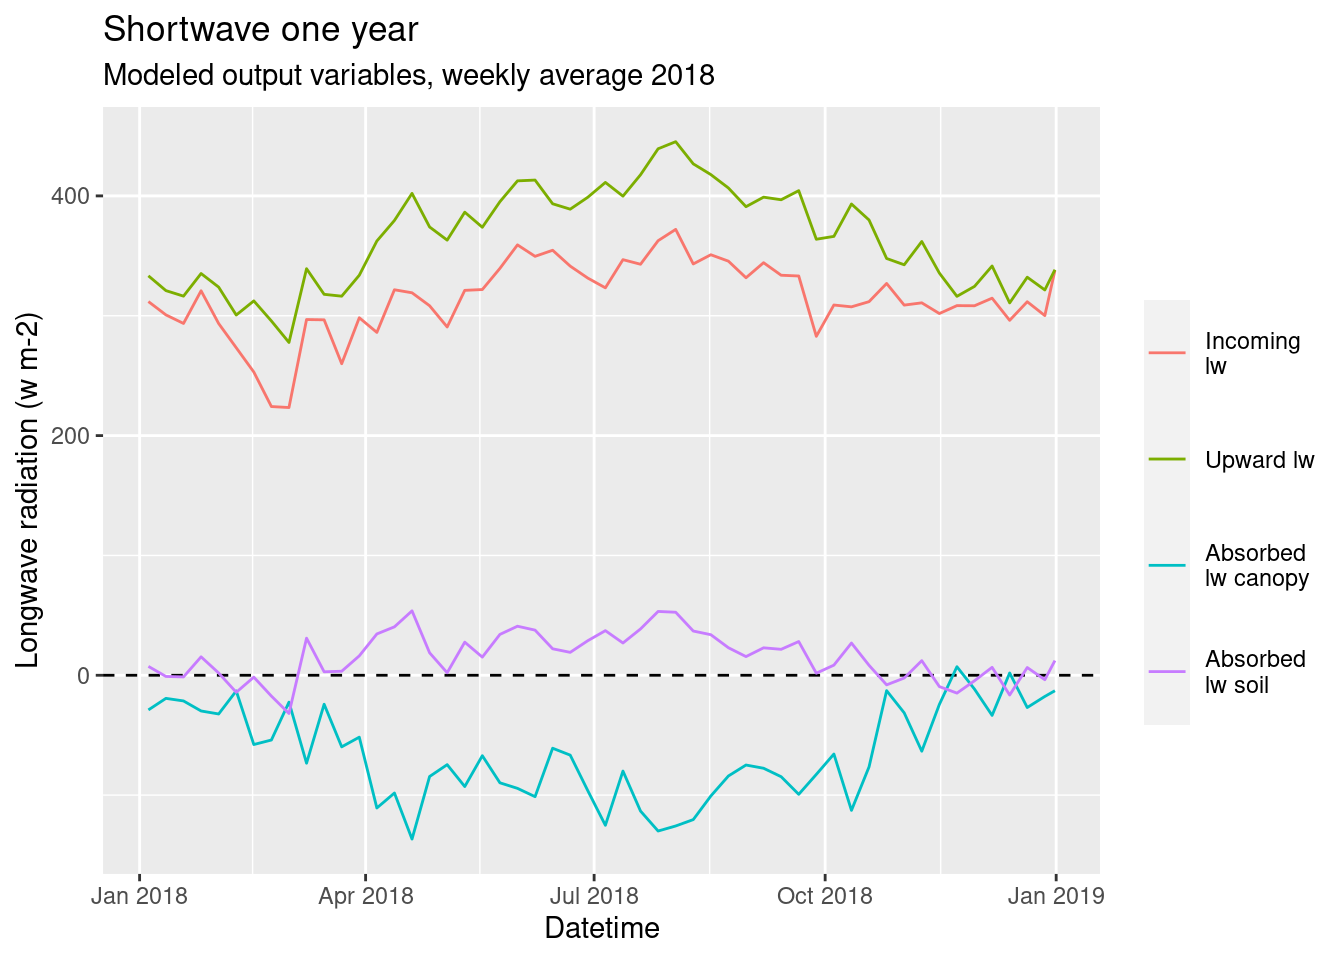
\includegraphics{SoilMoisture_Notebook_files/figure-latex/unnamed-chunk-6-1.pdf}

\hypertarget{calibration}{%
\section{4. Calibration}\label{calibration}}

Calibration was done for

\begin{verbatim}
  - saturated soil water content (theta.sat) [m3 m-3]
  - exponent for soil hydraulic equations (b.sm) [unitless]
\end{verbatim}

\begin{Shaded}
\begin{Highlighting}[]
\KeywordTok{rm}\NormalTok{(}\DataTypeTok{list =} \KeywordTok{ls}\NormalTok{())}

\NormalTok{parsfile <-}\StringTok{ "pars_soil.csv"}

\NormalTok{pars_calib <-}\StringTok{ }\KeywordTok{c}\NormalTok{(}\DataTypeTok{b.sm =} \FloatTok{11.4}\NormalTok{, }\DataTypeTok{theta.sat =} \FloatTok{0.48}\NormalTok{)}
\NormalTok{pars_low <-}\StringTok{ }\KeywordTok{c}\NormalTok{(}\DataTypeTok{b.sm =} \DecValTok{5}\NormalTok{, }\DataTypeTok{theta.sat =} \FloatTok{0.3}\NormalTok{)}
\NormalTok{pars_high <-}\StringTok{ }\KeywordTok{c}\NormalTok{(}\DataTypeTok{b.sm =} \DecValTok{13}\NormalTok{, }\DataTypeTok{theta.sat =} \FloatTok{0.6}\NormalTok{)}

\KeywordTok{source}\NormalTok{(}\StringTok{"setup_soilmoisture.R"}\NormalTok{)}
\KeywordTok{source}\NormalTok{(}\StringTok{"fun_soilmoisture.R"}\NormalTok{)}
\KeywordTok{source}\NormalTok{(}\StringTok{"fun_costmoisture.R"}\NormalTok{)}

\NormalTok{myfit <-}\StringTok{ }\KeywordTok{modFit}\NormalTok{(}\DataTypeTok{f =}\NormalTok{ cost_soilmoisture, }\DataTypeTok{p =}\NormalTok{ pars_calib, }\DataTypeTok{lower =}\NormalTok{ pars_low, }\DataTypeTok{upper =}\NormalTok{ pars_high)}
\end{Highlighting}
\end{Shaded}

\begin{verbatim}
##      b.sm theta.sat 
##     11.40      0.48 
##      b.sm theta.sat 
##     11.40      0.48 
##      b.sm theta.sat 
##     11.40      0.48 
##      b.sm theta.sat 
##     11.40      0.48 
##      b.sm theta.sat 
## 5.2464458 0.5812737 
##       b.sm  theta.sat 
## 11.0963809  0.5226837 
##       b.sm  theta.sat 
## 11.0963809  0.5226837 
##       b.sm  theta.sat 
## 11.0963809  0.5226837 
##      b.sm theta.sat 
## 9.3951653 0.5581726 
##       b.sm  theta.sat 
## 11.3217878  0.5261235 
##       b.sm  theta.sat 
## 11.3217878  0.5261235 
##       b.sm  theta.sat 
## 11.3217878  0.5261235 
##       b.sm  theta.sat 
## 11.0706687  0.5360297 
##       b.sm  theta.sat 
## 11.2293077  0.5315557 
##       b.sm  theta.sat 
## 11.2293077  0.5315557 
##       b.sm  theta.sat 
## 11.2293077  0.5315557 
##       b.sm  theta.sat 
## 10.9733276  0.5403582 
##       b.sm  theta.sat 
## 11.2044781  0.5330697 
##       b.sm  theta.sat 
## 11.2044781  0.5330697 
##       b.sm  theta.sat 
## 11.2044781  0.5330697 
##       b.sm  theta.sat 
## 11.1399991  0.5355971 
##       b.sm  theta.sat 
## 11.1399991  0.5355971 
##       b.sm  theta.sat 
## 11.1399991  0.5355971 
##       b.sm  theta.sat 
## 11.0232043  0.5401098 
##       b.sm  theta.sat 
## 11.0232043  0.5401098 
##       b.sm  theta.sat 
## 11.0232043  0.5401098 
##      b.sm theta.sat 
##  10.92661   0.54439 
##      b.sm theta.sat 
##  10.92661   0.54439 
##      b.sm theta.sat 
##  10.92661   0.54439 
##       b.sm  theta.sat 
## 10.8428641  0.5481948 
##       b.sm  theta.sat 
## 10.8428641  0.5481948 
##       b.sm  theta.sat 
## 10.8428641  0.5481948 
##       b.sm  theta.sat 
## 10.7696553  0.5515805 
##       b.sm  theta.sat 
## 10.7696553  0.5515805 
##       b.sm  theta.sat 
## 10.7696553  0.5515805 
##       b.sm  theta.sat 
## 10.6314394  0.5572772 
##       b.sm  theta.sat 
## 10.7208880  0.5539831 
##       b.sm  theta.sat 
## 10.7208880  0.5539831 
##       b.sm  theta.sat 
## 10.7208880  0.5539831 
##       b.sm  theta.sat 
## 10.6227938  0.5581803 
##       b.sm  theta.sat 
## 10.6227939  0.5581803 
##       b.sm  theta.sat 
## 10.6227938  0.5581803 
##       b.sm  theta.sat 
## 10.5519833  0.5617472 
##       b.sm  theta.sat 
## 10.5519833  0.5617472 
##       b.sm  theta.sat 
## 10.5519833  0.5617472 
##       b.sm  theta.sat 
## 10.4916848  0.5647879 
##       b.sm  theta.sat 
## 10.4916848  0.5647879 
##       b.sm  theta.sat 
## 10.4916848  0.5647879 
##       b.sm  theta.sat 
## 10.3812722  0.5696672 
##       b.sm  theta.sat 
## 10.4504568  0.5669787 
##       b.sm  theta.sat 
## 10.4504568  0.5669787 
##       b.sm  theta.sat 
## 10.4504568  0.5669787 
##       b.sm  theta.sat 
## 10.3699231  0.5706573 
##       b.sm  theta.sat 
## 10.3699231  0.5706573 
##       b.sm  theta.sat 
## 10.3699231  0.5706573 
##       b.sm  theta.sat 
## 10.3157271  0.5736259 
##       b.sm  theta.sat 
## 10.3157271  0.5736259 
##       b.sm  theta.sat 
## 10.3157271  0.5736259 
##       b.sm  theta.sat 
## 10.2709214  0.5760625 
##       b.sm  theta.sat 
## 10.2709214  0.5760625 
##       b.sm  theta.sat 
## 10.2709214  0.5760625 
##      b.sm theta.sat 
## 10.190602  0.579814 
##       b.sm  theta.sat 
## 10.2365652  0.5779693 
##       b.sm  theta.sat 
## 10.2365652  0.5779693 
##       b.sm  theta.sat 
## 10.2365652  0.5779693 
##       b.sm  theta.sat 
## 10.1730259  0.5810078 
##       b.sm  theta.sat 
## 10.1730259  0.5810078 
##       b.sm  theta.sat 
## 10.1730259  0.5810078 
##       b.sm  theta.sat 
## 10.1341922  0.5833188 
##       b.sm  theta.sat 
## 10.1341922  0.5833188 
##       b.sm  theta.sat 
## 10.1341922  0.5833188 
##       b.sm  theta.sat 
## 10.1030609  0.5851327 
##       b.sm  theta.sat 
## 10.1030609  0.5851327 
##       b.sm  theta.sat 
## 10.1030609  0.5851327 
##       b.sm  theta.sat 
## 10.0481876  0.5877939 
##       b.sm  theta.sat 
## 10.0481876  0.5877939 
##       b.sm  theta.sat 
## 10.0481876  0.5877939 
##       b.sm  theta.sat 
## 10.0397031  0.5887983 
##       b.sm  theta.sat 
## 10.0397031  0.5887983 
##       b.sm  theta.sat 
## 10.0397031  0.5887983 
##       b.sm  theta.sat 
## 10.0084029  0.5903827 
##       b.sm  theta.sat 
## 10.0084029  0.5903827 
##       b.sm  theta.sat 
## 10.0084029  0.5903827 
##      b.sm theta.sat 
## 9.9891623 0.5915755 
##      b.sm theta.sat 
## 9.9891623 0.5915755 
##      b.sm theta.sat 
## 9.9891623 0.5915755 
##      b.sm theta.sat 
##  9.955427  0.593251 
##      b.sm theta.sat 
##  9.955427  0.593251 
##      b.sm theta.sat 
##  9.955427  0.593251 
##      b.sm theta.sat 
## 9.9512012 0.5938618 
##      b.sm theta.sat 
## 9.9512012 0.5938618 
##      b.sm theta.sat 
## 9.9512012 0.5938618 
##      b.sm theta.sat 
## 9.9329830 0.5948028 
##      b.sm theta.sat 
## 9.9329830 0.5948028 
##      b.sm theta.sat 
## 9.9329830 0.5948028 
##      b.sm theta.sat 
## 9.9222191 0.5954938 
##      b.sm theta.sat 
## 9.9222191 0.5954938 
##      b.sm theta.sat 
## 9.9222191 0.5954938 
##      b.sm theta.sat 
## 9.9034412 0.5964406 
##      b.sm theta.sat 
## 9.9034412 0.5964406 
##      b.sm theta.sat 
## 9.9034412 0.5964406 
##      b.sm theta.sat 
## 9.8950051 0.5970587 
##      b.sm theta.sat 
## 9.8950051 0.5970587 
##      b.sm theta.sat 
## 9.8950051 0.5970587 
##      b.sm theta.sat 
##  9.879805  0.597817 
##      b.sm theta.sat 
##  9.879805  0.597817 
##      b.sm theta.sat 
##  9.879805  0.597817 
##      b.sm theta.sat 
## 9.8747425 0.5982645 
##      b.sm theta.sat 
## 9.8747425 0.5982645 
##      b.sm theta.sat 
## 9.8747425 0.5982645 
##      b.sm theta.sat 
## 9.8646447 0.5987691 
##      b.sm theta.sat 
## 9.8646447 0.5987691 
##      b.sm theta.sat 
## 9.8646447 0.5987691 
##      b.sm theta.sat 
## 9.8620908 0.5990464 
##      b.sm theta.sat 
## 9.8620909 0.5990464 
##      b.sm theta.sat 
## 9.8620908 0.5990464 
##      b.sm theta.sat 
## 9.8562029 0.5993426 
##      b.sm theta.sat 
## 9.8562029 0.5993426 
##      b.sm theta.sat 
## 9.8562029 0.5993426 
##      b.sm theta.sat 
## 9.8550017 0.5994984 
##      b.sm theta.sat 
## 9.8550017 0.5994984 
##      b.sm theta.sat 
## 9.8550017 0.5994984 
##      b.sm theta.sat 
## 9.8518153 0.5996597 
##      b.sm theta.sat 
## 9.8518154 0.5996597 
##      b.sm theta.sat 
## 9.8518153 0.5996597 
##      b.sm theta.sat 
## 9.8512525 0.5997425 
##      b.sm theta.sat 
## 9.8512525 0.5997425 
##      b.sm theta.sat 
## 9.8512525 0.5997425 
##      b.sm theta.sat 
## 9.8495945 0.5998268 
##      b.sm theta.sat 
## 9.8495945 0.5998268 
##      b.sm theta.sat 
## 9.8495945 0.5998268 
##      b.sm theta.sat 
## 9.8493256 0.5998695 
##      b.sm theta.sat 
## 9.8493256 0.5998695 
##      b.sm theta.sat 
## 9.8493256 0.5998695 
##      b.sm theta.sat 
## 9.8484798 0.5999126 
##      b.sm theta.sat 
## 9.8484798 0.5999126 
##      b.sm theta.sat 
## 9.8484798 0.5999126 
##      b.sm theta.sat 
## 9.8483490 0.5999343 
##      b.sm theta.sat 
## 9.8483490 0.5999343 
##      b.sm theta.sat 
## 9.8483490 0.5999343 
##      b.sm theta.sat 
## 9.8479214 0.5999561 
##      b.sm theta.sat 
## 9.8479214 0.5999561 
##      b.sm theta.sat 
## 9.8479214 0.5999561 
##      b.sm theta.sat 
##  9.847857  0.599967 
##      b.sm theta.sat 
##  9.847857  0.599967 
##      b.sm theta.sat 
##  9.847857  0.599967 
##      b.sm theta.sat 
##  9.847643  0.599978 
##      b.sm theta.sat 
##  9.847643  0.599978 
##      b.sm theta.sat 
##  9.847643  0.599978 
##      b.sm theta.sat 
## 9.8476106 0.5999835 
##      b.sm theta.sat 
## 9.8476106 0.5999835 
##      b.sm theta.sat 
## 9.8476106 0.5999835 
##      b.sm theta.sat 
## 9.8475721 0.5999868 
##      b.sm theta.sat 
## 9.8475721 0.5999868 
##      b.sm theta.sat 
## 9.8475721 0.5999868 
##      b.sm theta.sat 
## 9.8474973 0.5999906 
##      b.sm theta.sat 
## 9.8474973 0.5999906 
##      b.sm theta.sat 
## 9.8474973 0.5999906 
##      b.sm theta.sat 
## 9.8474771 0.5999927 
##      b.sm theta.sat 
## 9.8474771 0.5999927 
##      b.sm theta.sat 
## 9.8474771 0.5999927 
##      b.sm theta.sat 
##  9.847460  0.599994 
##      b.sm theta.sat 
##  9.847460  0.599994 
##      b.sm theta.sat 
##  9.847460  0.599994 
##      b.sm theta.sat 
## 9.8474280 0.5999956 
##      b.sm theta.sat 
## 9.8474280 0.5999956 
##      b.sm theta.sat 
## 9.8474280 0.5999956 
##      b.sm theta.sat 
## 9.8474179 0.5999965 
##      b.sm theta.sat 
## 9.8474179 0.5999965 
##      b.sm theta.sat 
## 9.8474179 0.5999965 
##      b.sm theta.sat 
## 9.8474098 0.5999971 
##      b.sm theta.sat 
## 9.8474098 0.5999971 
##      b.sm theta.sat 
## 9.8474098 0.5999971 
##      b.sm theta.sat 
## 9.8473951 0.5999979 
##      b.sm theta.sat 
## 9.8473951 0.5999979 
##      b.sm theta.sat 
## 9.8473951 0.5999979 
##      b.sm theta.sat 
## 9.8473826 0.5999985 
##      b.sm theta.sat 
## 9.8473826 0.5999985 
##      b.sm theta.sat 
## 9.8473826 0.5999985 
##      b.sm theta.sat 
## 9.8473794 0.5999989 
##      b.sm theta.sat 
## 9.8473794 0.5999989 
##      b.sm theta.sat 
## 9.8473794 0.5999989 
##      b.sm theta.sat 
## 9.8473721 0.5999993 
##      b.sm theta.sat 
## 9.8473721 0.5999993 
##      b.sm theta.sat 
## 9.8473721 0.5999993 
##      b.sm theta.sat 
## 9.8473675 0.5999996 
##      b.sm theta.sat 
## 9.8473675 0.5999996 
##      b.sm theta.sat 
## 9.8473675 0.5999996 
##      b.sm theta.sat 
## 9.8473691 0.5999997 
##      b.sm theta.sat 
## 9.8473691 0.5999997 
##      b.sm theta.sat 
## 9.8473691 0.5999997 
##      b.sm theta.sat 
## 9.8473698 0.5999996 
##      b.sm theta.sat 
## 9.8473695 0.5999996 
##      b.sm theta.sat 
## 9.8473691 0.5999997 
##      b.sm theta.sat 
## 9.8473692 0.5999997 
##      b.sm theta.sat 
## 9.8473690 0.5999997 
##      b.sm theta.sat 
## 9.8473691 0.5999997 
##      b.sm theta.sat 
## 9.8473691 0.5999996
\end{verbatim}

\begin{Shaded}
\begin{Highlighting}[]
\KeywordTok{summary}\NormalTok{(myfit)}
\end{Highlighting}
\end{Shaded}

\begin{verbatim}
## 
## Parameters:
##           Estimate Std. Error t value Pr(>|t|)    
## b.sm        9.8474     1.0150   9.702   <2e-16 ***
## theta.sat   0.6000     0.0606   9.900   <2e-16 ***
## ---
## Signif. codes:  0 '***' 0.001 '**' 0.01 '*' 0.05 '.' 0.1 ' ' 1
## 
## Residual standard error: 0.005995 on 742 degrees of freedom
## 
## Parameter correlation:
##              b.sm theta.sat
## b.sm       1.0000   -0.9999
## theta.sat -0.9999    1.0000
\end{verbatim}

\hypertarget{output}{%
\section{4. Output}\label{output}}

\hypertarget{run-model}{%
\subsubsection{4.1 Run model}\label{run-model}}

Finally, we run the model with the calibrated parameters and visualize
the output.

\begin{Shaded}
\begin{Highlighting}[]
\CommentTok{## Run model ##}


\CommentTok{# Run model with uncalibrated parameters}

\NormalTok{parsfile <-}\StringTok{ "pars_soil.csv"}
\KeywordTok{source}\NormalTok{(}\StringTok{"setup_soilmoisture.R"}\NormalTok{)}
\KeywordTok{source}\NormalTok{(}\StringTok{"fun_soilmoisture.R"}\NormalTok{)}

\NormalTok{output <-}\StringTok{ }\KeywordTok{get_theta_soil}\NormalTok{(}\DataTypeTok{input =}\NormalTok{ input, }\DataTypeTok{pars =}\NormalTok{ pars, }\DataTypeTok{initial_state =}\NormalTok{ initial_state)}


\CommentTok{# Run model choosing calibrated parameter file}

\NormalTok{parsfile <-}\StringTok{ "pars_soil_calib1.csv"}
\NormalTok{pars_soil_calib1 <-}\StringTok{ }\KeywordTok{read.csv}\NormalTok{(parsfile)}

\NormalTok{pars_soil_calib1[}\DecValTok{2}\NormalTok{,}\DecValTok{2}\NormalTok{] <-}\StringTok{ }\FloatTok{9.85}
\NormalTok{pars_soil_calib1[}\DecValTok{33}\NormalTok{,}\DecValTok{2}\NormalTok{] <-}\StringTok{ }\FloatTok{0.6}


\KeywordTok{source}\NormalTok{(}\StringTok{"setup_soilmoisture.R"}\NormalTok{)}
\KeywordTok{source}\NormalTok{(}\StringTok{"fun_soilmoisture.R"}\NormalTok{)}

\NormalTok{output_cal <-}\StringTok{ }\KeywordTok{get_theta_soil}\NormalTok{(}\DataTypeTok{input =}\NormalTok{ input, }\DataTypeTok{pars =}\NormalTok{ pars, }\DataTypeTok{initial_state =}\NormalTok{ initial_state)}
\end{Highlighting}
\end{Shaded}

\hypertarget{plotting}{%
\subsubsection{4.2 Plotting}\label{plotting}}

\begin{Shaded}
\begin{Highlighting}[]
\CommentTok{## Plotting ##}

\KeywordTok{library}\NormalTok{(ggplot2)}
\KeywordTok{library}\NormalTok{(gridExtra)}
\KeywordTok{library}\NormalTok{(tidyr)}


\CommentTok{# Compare measured data to modeled data and pre-calibrated data}

\NormalTok{out_theta <-}\StringTok{ }\KeywordTok{data.frame}\NormalTok{(fluxes}\OperatorTok{$}\NormalTok{time, fluxes}\OperatorTok{$}\NormalTok{swc, output_cal}\OperatorTok{$}\NormalTok{theta, output}\OperatorTok{$}\NormalTok{theta)}
\KeywordTok{names}\NormalTok{(out_theta) <-}\StringTok{ }\KeywordTok{c}\NormalTok{(}\StringTok{"time"}\NormalTok{, }\StringTok{"swc"}\NormalTok{, }\StringTok{"theta_cal"}\NormalTok{, }\StringTok{"theta"}\NormalTok{)}

\NormalTok{gg_theta <-}\StringTok{ }\KeywordTok{gather}\NormalTok{(out_theta, }\DataTypeTok{key =} \StringTok{"type"}\NormalTok{, }\DataTypeTok{value =} \StringTok{"theta"}\NormalTok{, swc, theta_cal, theta, }\DataTypeTok{factor_key =}\NormalTok{ T)}

\KeywordTok{ggplot}\NormalTok{() }\OperatorTok{+}
\StringTok{  }\KeywordTok{geom_line}\NormalTok{(}\KeywordTok{aes}\NormalTok{(gg_theta}\OperatorTok{$}\NormalTok{time, gg_theta}\OperatorTok{$}\NormalTok{theta, }\DataTypeTok{color =}\NormalTok{ gg_theta}\OperatorTok{$}\NormalTok{type), }\DataTypeTok{size =} \DecValTok{1}\NormalTok{) }\OperatorTok{+}
\StringTok{  }\KeywordTok{labs}\NormalTok{(}\DataTypeTok{y =} \StringTok{"soil water content [m3 m-3]"}\NormalTok{, }\DataTypeTok{x =} \StringTok{"time"}\NormalTok{, }\DataTypeTok{color =} \StringTok{""}\NormalTok{)}
\end{Highlighting}
\end{Shaded}

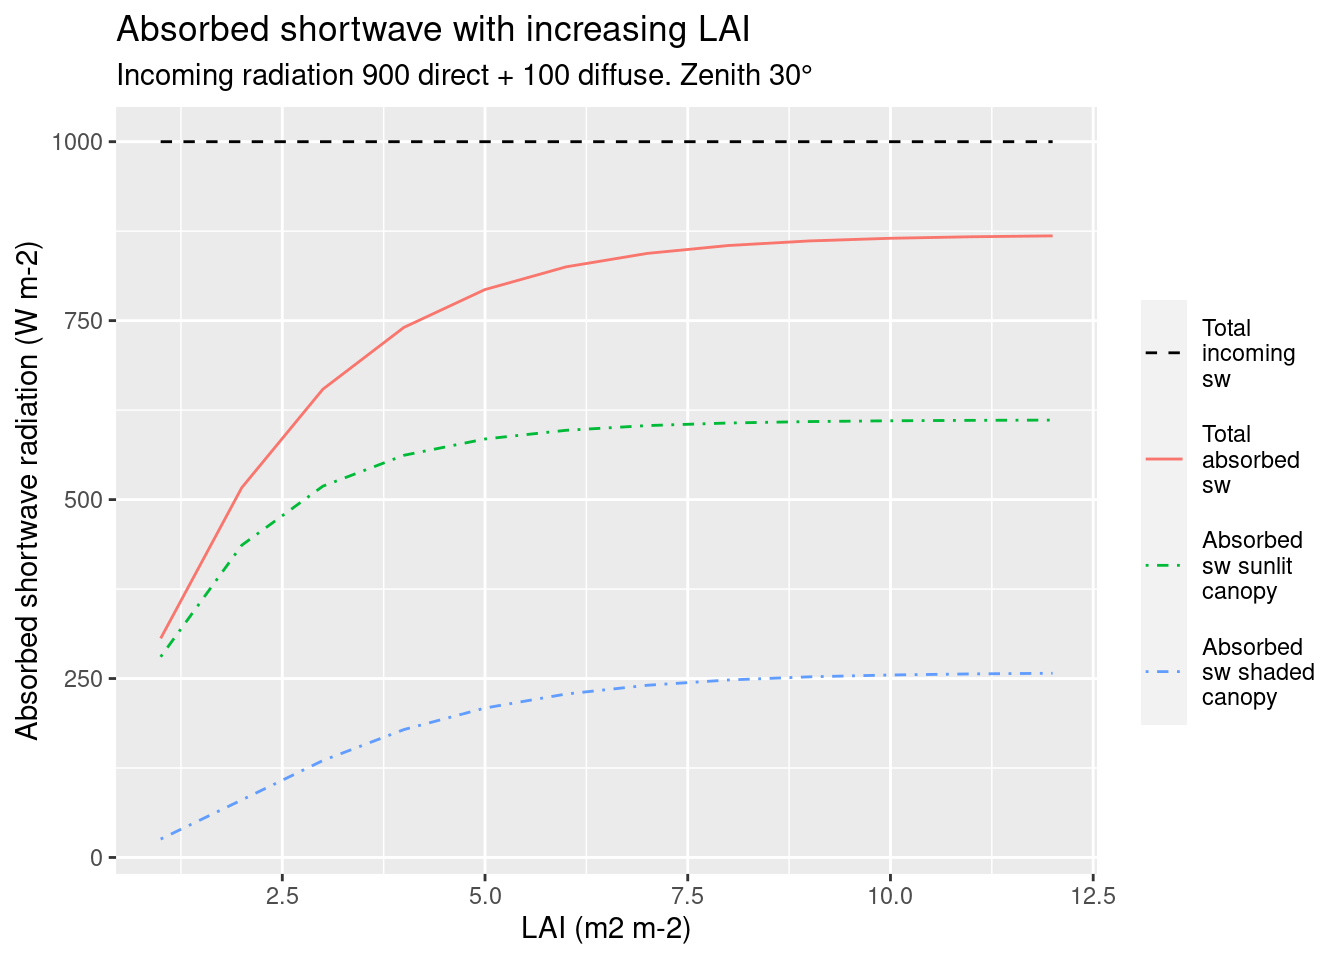
\includegraphics{SoilMoisture_Notebook_files/figure-latex/unnamed-chunk-9-1.pdf}

\begin{Shaded}
\begin{Highlighting}[]
\CommentTok{# Plotting output variables}

\NormalTok{out <-}\StringTok{ }\KeywordTok{data.frame}\NormalTok{(fluxes}\OperatorTok{$}\NormalTok{time, output_cal[ , }\DecValTok{-8}\NormalTok{], input}\OperatorTok{$}\NormalTok{p)}
\KeywordTok{names}\NormalTok{(out) <-}\StringTok{ }\KeywordTok{c}\NormalTok{(}\StringTok{"time"}\NormalTok{, }\StringTok{"theta"}\NormalTok{, }\StringTok{"runoff"}\NormalTok{, }\StringTok{"hyd_conductivity"}\NormalTok{, }\StringTok{"evaporation"}\NormalTok{, }\StringTok{"drainage"}\NormalTok{, }\StringTok{"water_potential"}\NormalTok{, }\StringTok{"water_potential_sub"}\NormalTok{, }\StringTok{"precipitation"}\NormalTok{)}


\CommentTok{# evaporation}

\NormalTok{gg_theta <-}\StringTok{ }\KeywordTok{gather}\NormalTok{(out, }\DataTypeTok{key =} \StringTok{"type"}\NormalTok{, }\DataTypeTok{value =} \StringTok{"theta"}\NormalTok{, evaporation, }\DataTypeTok{factor_key =}\NormalTok{ T)}

\KeywordTok{ggplot}\NormalTok{() }\OperatorTok{+}
\StringTok{  }\KeywordTok{geom_line}\NormalTok{(}\KeywordTok{aes}\NormalTok{(gg_theta}\OperatorTok{$}\NormalTok{time, gg_theta}\OperatorTok{$}\NormalTok{theta, }\DataTypeTok{color =}\NormalTok{ gg_theta}\OperatorTok{$}\NormalTok{type), }\DataTypeTok{size =} \DecValTok{1}\NormalTok{) }\OperatorTok{+}
\StringTok{  }\KeywordTok{labs}\NormalTok{(}\DataTypeTok{y =} \StringTok{"evaporation [m s-1]"}\NormalTok{, }\DataTypeTok{x =} \StringTok{"time"}\NormalTok{, }\DataTypeTok{color =} \StringTok{""}\NormalTok{)}
\end{Highlighting}
\end{Shaded}

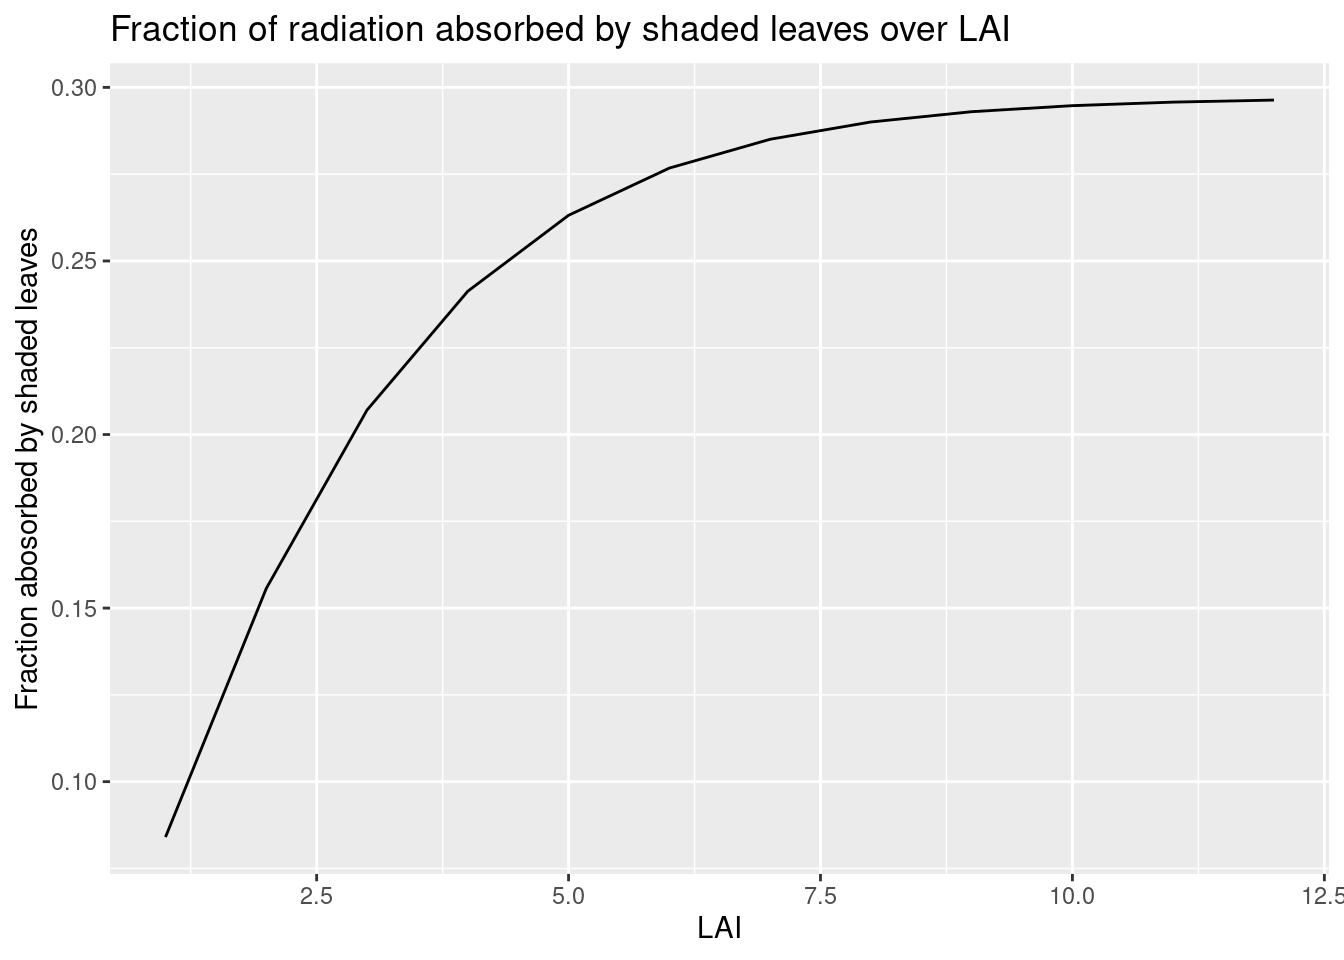
\includegraphics{SoilMoisture_Notebook_files/figure-latex/unnamed-chunk-10-1.pdf}

\begin{Shaded}
\begin{Highlighting}[]
\CommentTok{# drainage against hydraulic conductivity}

\NormalTok{gg_theta <-}\StringTok{ }\KeywordTok{gather}\NormalTok{(out, }\DataTypeTok{key =} \StringTok{"type"}\NormalTok{, }\DataTypeTok{value =} \StringTok{"theta"}\NormalTok{, drainage, }\DataTypeTok{factor_key =}\NormalTok{ T)}

\KeywordTok{ggplot}\NormalTok{() }\OperatorTok{+}
\StringTok{  }\KeywordTok{geom_line}\NormalTok{(}\KeywordTok{aes}\NormalTok{(gg_theta}\OperatorTok{$}\NormalTok{hyd_conductivity, gg_theta}\OperatorTok{$}\NormalTok{theta, }\DataTypeTok{color =}\NormalTok{ gg_theta}\OperatorTok{$}\NormalTok{type), }\DataTypeTok{size =} \DecValTok{1}\NormalTok{) }\OperatorTok{+}
\StringTok{  }\KeywordTok{labs}\NormalTok{(}\DataTypeTok{y =} \StringTok{"drainage [m s-1]"}\NormalTok{, }\DataTypeTok{x =} \StringTok{"hydraulic conductivity [m s-1]"}\NormalTok{, }\DataTypeTok{color =} \StringTok{""}\NormalTok{)}
\end{Highlighting}
\end{Shaded}

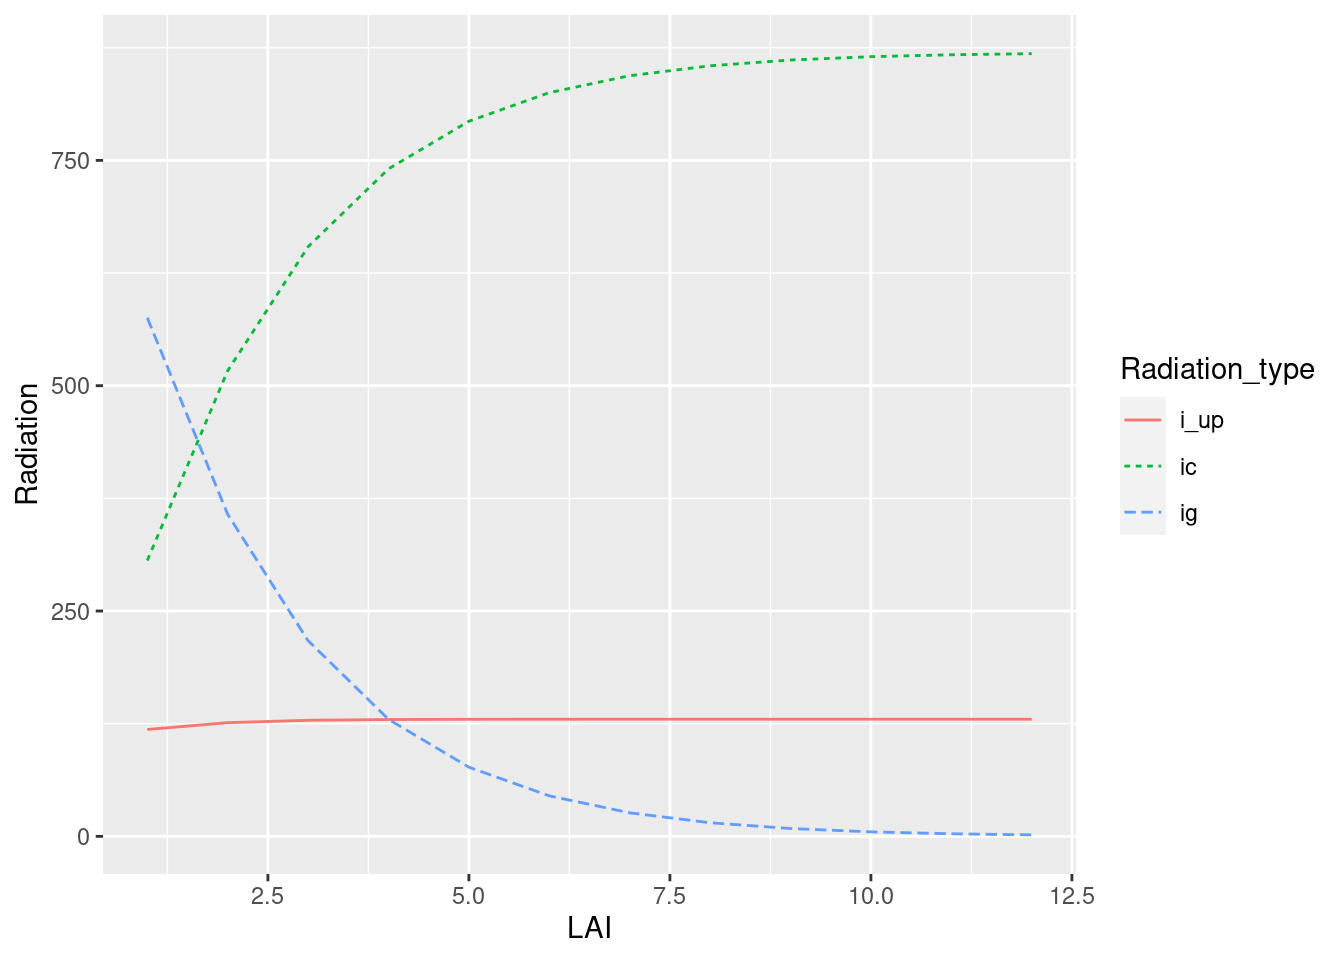
\includegraphics{SoilMoisture_Notebook_files/figure-latex/unnamed-chunk-11-1.pdf}

\begin{Shaded}
\begin{Highlighting}[]
\CommentTok{# water potential and precipitation}

\NormalTok{gg_thetaWP <-}\StringTok{ }\KeywordTok{gather}\NormalTok{(out, }\DataTypeTok{key =} \StringTok{"type"}\NormalTok{, }\DataTypeTok{value =} \StringTok{"theta"}\NormalTok{, water_potential, }\DataTypeTok{factor_key =}\NormalTok{ T)}

\NormalTok{WP <-}\StringTok{ }\KeywordTok{ggplot}\NormalTok{() }\OperatorTok{+}
\StringTok{  }\KeywordTok{geom_line}\NormalTok{(}\KeywordTok{aes}\NormalTok{(gg_thetaWP}\OperatorTok{$}\NormalTok{time, gg_thetaWP}\OperatorTok{$}\NormalTok{theta, }\DataTypeTok{color =}\NormalTok{ gg_thetaWP}\OperatorTok{$}\NormalTok{type), }\DataTypeTok{size =} \DecValTok{1}\NormalTok{) }\OperatorTok{+}
\StringTok{  }\KeywordTok{labs}\NormalTok{(}\DataTypeTok{y =} \StringTok{"water potential [m]"}\NormalTok{, }\DataTypeTok{x =} \StringTok{"time"}\NormalTok{, }\DataTypeTok{color =} \StringTok{""}\NormalTok{)}


\NormalTok{gg_thetaP <-}\StringTok{ }\KeywordTok{gather}\NormalTok{(out, }\DataTypeTok{key =} \StringTok{"type"}\NormalTok{, }\DataTypeTok{value =} \StringTok{"theta"}\NormalTok{, precipitation, }\DataTypeTok{factor_key =}\NormalTok{ T)}

\NormalTok{P <-}\StringTok{ }\KeywordTok{ggplot}\NormalTok{() }\OperatorTok{+}
\StringTok{  }\KeywordTok{geom_line}\NormalTok{(}\KeywordTok{aes}\NormalTok{(gg_thetaP}\OperatorTok{$}\NormalTok{time, gg_thetaP}\OperatorTok{$}\NormalTok{theta, }\DataTypeTok{color =}\NormalTok{ gg_thetaP}\OperatorTok{$}\NormalTok{type), }\DataTypeTok{size =} \DecValTok{1}\NormalTok{) }\OperatorTok{+}
\StringTok{  }\KeywordTok{labs}\NormalTok{(}\DataTypeTok{y =} \StringTok{"precipitation [m3 dt-1]"}\NormalTok{, }\DataTypeTok{x =} \StringTok{"time"}\NormalTok{, }\DataTypeTok{color =} \StringTok{""}\NormalTok{)}

\KeywordTok{grid.arrange}\NormalTok{(WP, P)}
\end{Highlighting}
\end{Shaded}

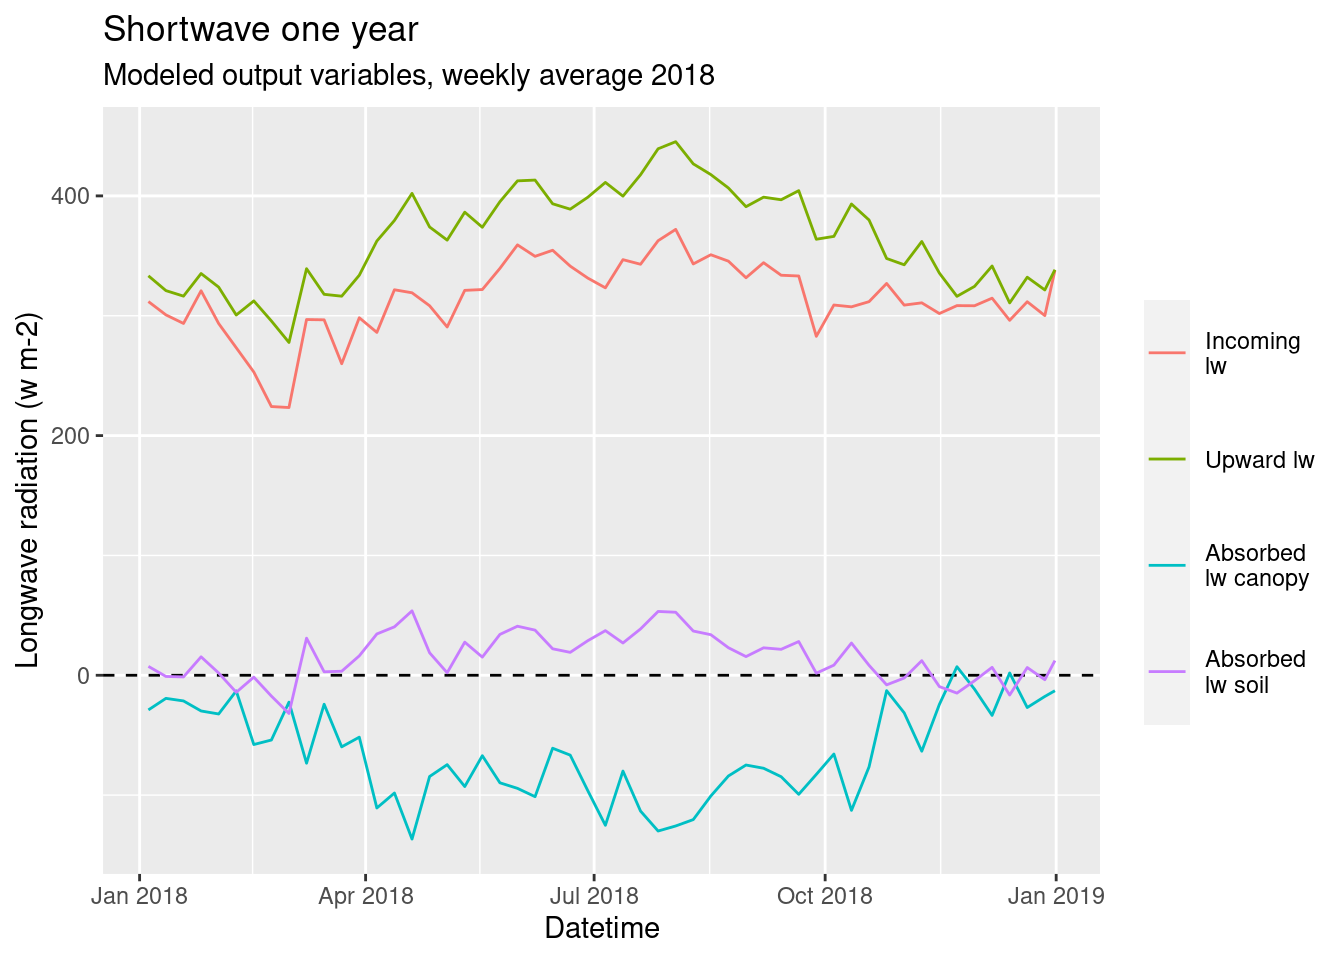
\includegraphics{SoilMoisture_Notebook_files/figure-latex/unnamed-chunk-12-1.pdf}

\begin{Shaded}
\begin{Highlighting}[]
\CommentTok{# multiple plots together for comparison}

\NormalTok{gg_thetaA <-}\StringTok{ }\KeywordTok{gather}\NormalTok{(out, }\DataTypeTok{key =} \StringTok{"type"}\NormalTok{, }\DataTypeTok{value =} \StringTok{"theta"}\NormalTok{, theta, }\DataTypeTok{factor_key =}\NormalTok{ T)}

\NormalTok{A <-}\StringTok{ }\KeywordTok{ggplot}\NormalTok{() }\OperatorTok{+}
\StringTok{  }\KeywordTok{geom_line}\NormalTok{(}\KeywordTok{aes}\NormalTok{(gg_thetaA}\OperatorTok{$}\NormalTok{time, gg_thetaA}\OperatorTok{$}\NormalTok{theta, }\DataTypeTok{color =}\NormalTok{ gg_thetaA}\OperatorTok{$}\NormalTok{type), }\DataTypeTok{size =} \DecValTok{1}\NormalTok{) }\OperatorTok{+}
\StringTok{  }\KeywordTok{labs}\NormalTok{(}\DataTypeTok{y =} \StringTok{"theta [m3 m-3]"}\NormalTok{, }\DataTypeTok{x =} \StringTok{"time"}\NormalTok{, }\DataTypeTok{color =} \StringTok{""}\NormalTok{)}

\NormalTok{gg_thetaB <-}\StringTok{ }\KeywordTok{gather}\NormalTok{(out, }\DataTypeTok{key =} \StringTok{"type"}\NormalTok{, }\DataTypeTok{value =} \StringTok{"theta"}\NormalTok{, precipitation, }\DataTypeTok{factor_key =}\NormalTok{ T)}

\NormalTok{B <-}\StringTok{ }\KeywordTok{ggplot}\NormalTok{() }\OperatorTok{+}
\StringTok{  }\KeywordTok{geom_line}\NormalTok{(}\KeywordTok{aes}\NormalTok{(gg_thetaB}\OperatorTok{$}\NormalTok{time, gg_thetaB}\OperatorTok{$}\NormalTok{theta, }\DataTypeTok{color =}\NormalTok{ gg_thetaB}\OperatorTok{$}\NormalTok{type), }\DataTypeTok{size =} \DecValTok{1}\NormalTok{) }\OperatorTok{+}
\StringTok{  }\KeywordTok{labs}\NormalTok{(}\DataTypeTok{y =} \StringTok{"precipitation [m3 dt-1]"}\NormalTok{, }\DataTypeTok{x =} \StringTok{"time"}\NormalTok{, }\DataTypeTok{color =} \StringTok{""}\NormalTok{)}

\NormalTok{gg_thetaC <-}\StringTok{ }\KeywordTok{gather}\NormalTok{(out, }\DataTypeTok{key =} \StringTok{"type"}\NormalTok{, }\DataTypeTok{value =} \StringTok{"theta"}\NormalTok{, water_potential, }\DataTypeTok{factor_key =}\NormalTok{ T)}

\NormalTok{C <-}\StringTok{ }\KeywordTok{ggplot}\NormalTok{() }\OperatorTok{+}
\StringTok{  }\KeywordTok{geom_line}\NormalTok{(}\KeywordTok{aes}\NormalTok{(gg_thetaC}\OperatorTok{$}\NormalTok{time, gg_thetaC}\OperatorTok{$}\NormalTok{theta, }\DataTypeTok{color =}\NormalTok{ gg_thetaC}\OperatorTok{$}\NormalTok{type), }\DataTypeTok{size =} \DecValTok{1}\NormalTok{) }\OperatorTok{+}
\StringTok{  }\KeywordTok{labs}\NormalTok{(}\DataTypeTok{y =} \StringTok{"water potential [m]"}\NormalTok{, }\DataTypeTok{x =} \StringTok{"time"}\NormalTok{, }\DataTypeTok{color =} \StringTok{""}\NormalTok{)}

\NormalTok{gg_thetaD <-}\StringTok{ }\KeywordTok{gather}\NormalTok{(out, }\DataTypeTok{key =} \StringTok{"type"}\NormalTok{, }\DataTypeTok{value =} \StringTok{"theta"}\NormalTok{, drainage, }\DataTypeTok{factor_key =}\NormalTok{ T)}

\NormalTok{D <-}\StringTok{ }\KeywordTok{ggplot}\NormalTok{() }\OperatorTok{+}
\StringTok{  }\KeywordTok{geom_line}\NormalTok{(}\KeywordTok{aes}\NormalTok{(gg_thetaD}\OperatorTok{$}\NormalTok{time, gg_thetaD}\OperatorTok{$}\NormalTok{theta, }\DataTypeTok{color =}\NormalTok{ gg_thetaD}\OperatorTok{$}\NormalTok{type), }\DataTypeTok{size =} \DecValTok{1}\NormalTok{) }\OperatorTok{+}
\StringTok{  }\KeywordTok{labs}\NormalTok{(}\DataTypeTok{y =} \StringTok{"drainage [m s-1]"}\NormalTok{, }\DataTypeTok{x =} \StringTok{"time"}\NormalTok{, }\DataTypeTok{color =} \StringTok{""}\NormalTok{)}

\NormalTok{gg_thetaE <-}\StringTok{ }\KeywordTok{gather}\NormalTok{(out, }\DataTypeTok{key =} \StringTok{"type"}\NormalTok{, }\DataTypeTok{value =} \StringTok{"theta"}\NormalTok{, hyd_conductivity, }\DataTypeTok{factor_key =}\NormalTok{ T)}

\NormalTok{E <-}\StringTok{ }\KeywordTok{ggplot}\NormalTok{() }\OperatorTok{+}
\StringTok{  }\KeywordTok{geom_line}\NormalTok{(}\KeywordTok{aes}\NormalTok{(gg_thetaE}\OperatorTok{$}\NormalTok{time, gg_thetaE}\OperatorTok{$}\NormalTok{theta, }\DataTypeTok{color =}\NormalTok{ gg_thetaE}\OperatorTok{$}\NormalTok{type), }\DataTypeTok{size =} \DecValTok{1}\NormalTok{) }\OperatorTok{+}
\StringTok{  }\KeywordTok{labs}\NormalTok{(}\DataTypeTok{y =} \StringTok{"hydraulic conductivity [m s-1]"}\NormalTok{, }\DataTypeTok{x =} \StringTok{"time"}\NormalTok{, }\DataTypeTok{color =} \StringTok{""}\NormalTok{)}

\KeywordTok{grid.arrange}\NormalTok{(A, B, C, D, E, }\DataTypeTok{ncol =} \DecValTok{2}\NormalTok{)}
\end{Highlighting}
\end{Shaded}

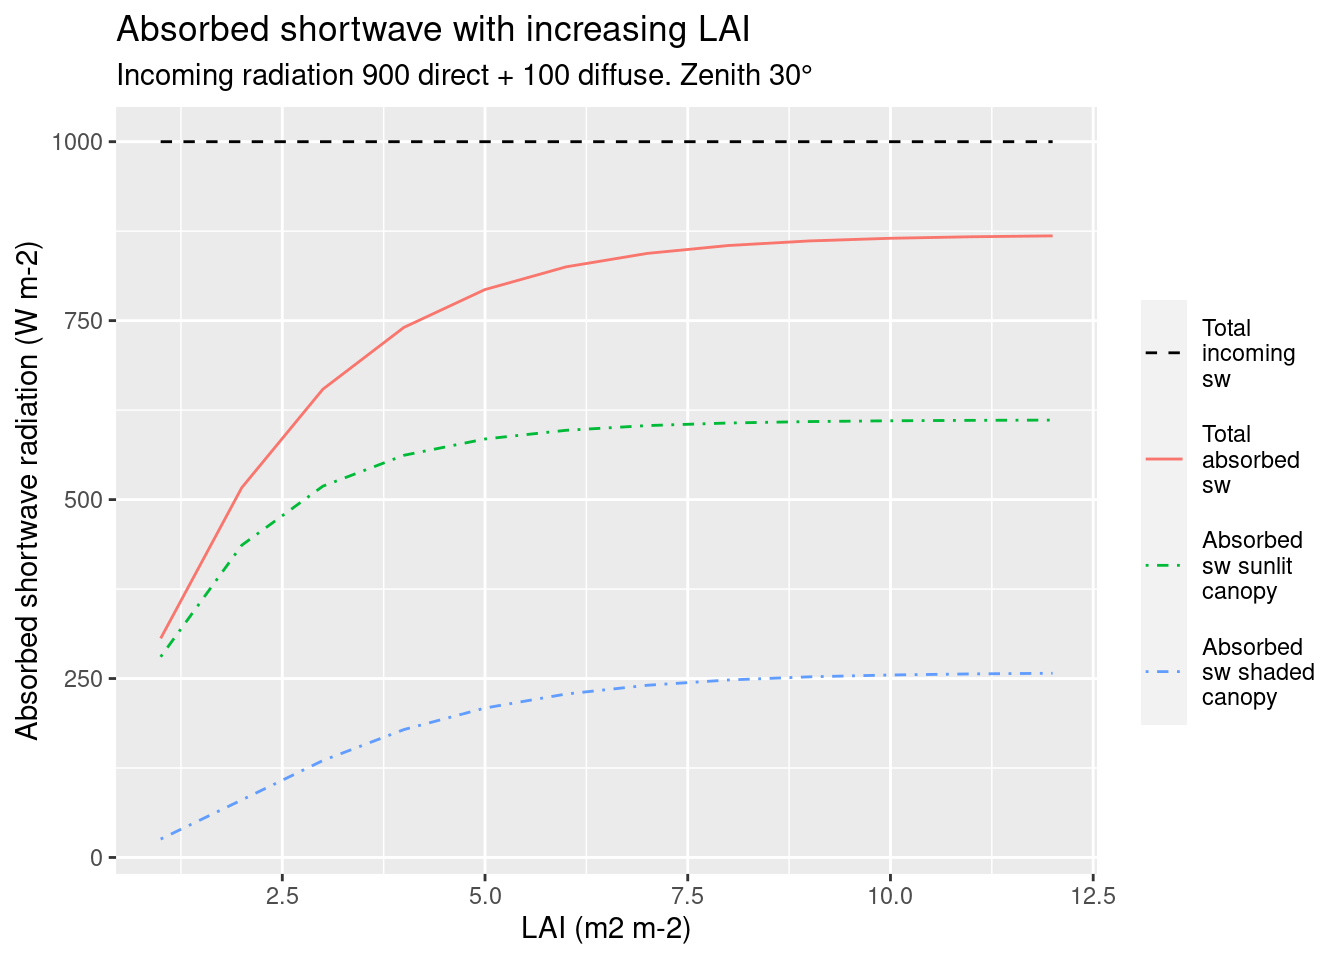
\includegraphics{SoilMoisture_Notebook_files/figure-latex/unnamed-chunk-13-1.pdf}

\end{document}
